\documentclass[11pt,a4paper]{article}
\usepackage[a4paper,left=20mm,right=20mm,top=20mm,bottom=20mm]{geometry}
\usepackage[T1]{fontenc}
\usepackage{lmodern,amsmath,amssymb,booktabs,array,tabularx,fancyhdr,graphicx}
\usepackage[british]{babel}
\usepackage[hidelinks]{hyperref}
\usepackage{caption,float,microtype,enumitem}
\hypersetup{pdftitle={OUC CW 1 38 - report draft},pdfauthor={Pinxin Liu and Chengtian Gong}}
\newcolumntype{Y}{>{\raggedright\arraybackslash}X}
\captionsetup{font=normalsize,labelfont=bf,skip=5pt}
\setlength{\parindent}{0pt}
\setlength{\parskip}{.45em}
\setlength{\headheight}{14pt}
\setlength{\emergencystretch}{2em}
\renewcommand{\arraystretch}{1.16}
\setlist[enumerate]{leftmargin=*,itemsep=2pt,topsep=4pt}
\pagestyle{fancy}\fancyhf{}
\fancyhead[C]{\small F29AI Coursework 1\quad OUC Group 38}
\fancyfoot[C]{\thepage}
\renewcommand{\headrulewidth}{0pt}
\renewcommand{\footrulewidth}{0pt}
\newcommand{\GroupName}{OUC CW 1 38}
\newcommand{\MemberRows}{Pinxin Liu & H00490337 & pl4005\\
Chengtian Gong & H00490375 & cg4005\\}
\newcommand{\VideoLink}{PENDING - both members must present; maximum eight minutes.}
\newcommand{\ReportStatus}{DRAFT - video link pending}

\title{Coursework 1 Report\\Search and Automated Planning}
\author{Pinxin Liu\quad Chengtian Gong\\\GroupName}
\date{28 October 2026}
\begin{document}
\pagenumbering{roman}
\begin{titlepage}
\maketitle\thispagestyle{plain}
\begin{center}\textbf{\ReportStatus}\end{center}
\begin{table}[H]\centering
\caption*{Group details}
\begin{tabularx}{\linewidth}{@{}Yrr@{}}
\toprule
\textbf{Member} & \textbf{HWU student ID} & \textbf{HWU username}\\
\midrule
\MemberRows
\bottomrule
\end{tabularx}
\end{table}
\medskip
\textbf{Video demonstration:} \VideoLink

\subsection*{Report structure and contributions}
Part 1 occupies pages \pageref{part1-start}--\pageref{part1-end}; Part 2 occupies pages \pageref{part2-start}--\pageref{part2-end}. The title page and reference list are separate. The report uses 11pt body text, a single column and 20mm margins.

Chengtian Gong: Part 1A and Parts 2A/2B. Pinxin Liu: Part 1B and Part 2C. Both members review the complete work and present substantial parts of the video.

Results refer to the saved experiment and validation records. The interface screenshot illustrates an interactive run; its displayed elapsed time is not substituted for the benchmark measurements.
\end{titlepage}
\pagenumbering{arabic}

\section{Part 1A: Sudoku as a CSP}\label{part1-start}
\subsection{Variables, domains and constraints}
A constraint satisfaction problem consists of variables, their domains and constraints on permitted assignments \cite{csp}. For the supplied $9\times9$ Sudoku \cite{spec}, define
\[
\mathcal{X}=\{X_{r,c}\mid r,c\in\{1,\ldots,9\}\},\qquad
D_{r,c}=\begin{cases}\{v\},&\text{if the given digit is }v,\\
\{1,\ldots,9\},&\text{if the cell is blank.}\end{cases}
\]
There is one variable per cell, hence 81 variables. Input zero denotes a blank; zero is never a solution value. Each given is fixed by its singleton domain. The 27 unit constraints are
\begin{align*}
&\operatorname{AllDifferent}(X_{r,1},\ldots,X_{r,9}) &&r=1,\ldots,9,\\
&\operatorname{AllDifferent}(X_{1,c},\ldots,X_{9,c}) &&c=1,\ldots,9,\\
&\operatorname{AllDifferent}\bigl((X_{3i+a,3j+b})_{a,b=1}^{3}\bigr)
&&i,j\in\{0,1,2\}.
\end{align*}
Together with the domains, these require every row, column and $3\times3$ box to contain each digit exactly once. A solution is a complete assignment satisfying every constraint and preserving all givens.

\subsection{Worst-case search and practical pruning}
Let $m$ be the number of initially blank cells. Brute force can enumerate $9^m$ complete digit assignments and check each completed grid. Backtracking assigns one blank at a time, checking partial consistency before descending \cite{csp,backtracking}. An unpruned tree with depth $m$ and branching factor at most nine contains at most
\[
\sum_{k=0}^{m}9^k=\frac{9^{m+1}-1}{8}=O(9^m)
\]
nodes. Thus both methods have a coarse exponential upper bound in $m$ when the cost of checking a fixed-size board is treated as constant. If checking work is counted separately, the node bound is multiplied by that cost. This comparison does not claim that backtracking has a polynomial worst case.

The practical advantage is \emph{early rejection}. Once a partial assignment contains a duplicate, assigning further cells cannot repair that duplicate. Rejecting a branch with $k$ blanks remaining can avoid up to $9^k$ complete extensions. A locally consistent branch can still fail later, so the amount saved depends on the puzzle and assignment order.

The chosen implementation adds minimum remaining values (MRV): select a blank with the fewest currently legal digits \cite{ordering}. A zero-candidate cell immediately exposes failure; a one-candidate cell is forced under the current assignment. MRV changes the order and size of the explored tree, while recomputing candidate sets adds work at each node. The comparison on page \pageref{evaluation} measures this trade-off rather than assuming MRV is always faster.

\clearpage
\section{Part 1B: Implementation and correctness}
\subsection{Method and design choices}
The implemented method is depth-first backtracking with MRV. It was chosen because it is complete over the finite legal assignment tree, needs no solver library, and has deterministic choices that make search counters reproducible. The board is a list of nine integer lists. \texttt{solve()} validates and copies the input, preserving the caller's board.

The \texttt{candidates()} function subtracts the digits present in a blank's row, column and box from $\{1,\ldots,9\}$. At every search call, MRV scans the blank cells and recomputes these sets. Ties are resolved in reading order, and digits are tried in ascending order. A fixed row-major ordering is available for a controlled comparison using the same solver and candidate rules.

\begin{enumerate}
\item Read nine rows from a TXT or CSV file; reject malformed values, shapes or conflicting givens.
\item At a search node, inspect the empty cells. If any inspected candidate set is empty, fail that branch.
\item If no blanks remain, return the completed board. Otherwise choose the MRV cell.
\item Assign each candidate in ascending order and recurse. On failure, reset that cell to zero before trying the next candidate.
\item If all candidates fail, return failure to the preceding call. Exhausting the root's choices reports no solution.
\end{enumerate}
Only the assigned cell needs undoing: the solver does not maintain propagated domains. In particular, it does not implement forward checking or AC-3. Candidate recomputation during selection should not be confused with maintaining filtered domains after every assignment.

\subsection{Input, output and interface}
The command \texttt{python3 solver.py puzzles/p2.txt --stats}, run in \texttt{reference/part1b}, displays a readable solution and optional counters. The CLI returns 0 for solved, 1 for a valid but unsatisfiable puzzle and 2 for an input error. TXT uses spaces and CSV uses commas, with zero for a blank.

The Tkinter interface shares the solver and validation code. Load reads a file, Solve searches, Reset restores the loaded original and Clear empties the board. Givens are black and added digits blue. The current interface also highlights duplicate values and displays candidates for a selected empty cell. Candidates express local legality, not a guarantee of a completion. Search is synchronous, so a demanding puzzle can temporarily block the window.

\subsection{Correctness checks and scope}
Seventeen solver tests cover parsing, invalid/conflicting input, several puzzles, completed and nearly completed boards, no-solution input, deterministic counters, input preservation and CLI return codes. A separate set-based oracle checks every returned row, column and box against $\{1,\ldots,9\}$ and verifies the givens. Six interface-state tests cover candidate display, conflicts, Clear and Reset; they use widget doubles, so native rendering and keyboard handling need an actual interface demonstration.

Finding one solution does not establish uniqueness. A separate \texttt{count\_solutions()} search stops after two completions; tests check one completion for the solvable practice inputs. The solver's finite exhaustive search is complete, but its exponential worst case limits practical performance.

\clearpage
\subsection{Quantitative evaluation}\label{evaluation}
Saved runs used CPython 3.9.6 on Darwin 27.0.0 arm64: five repetitions per input and ordering, in one process, without warm-up. Timing covers the complete \texttt{solve()} call, including validation and copying; file reading, earlier input validation, output and independent checking are excluded. Both orderings use identical input files and the same solver. All five inputs were constructed locally; no certified difficulty levels are claimed.

\begin{table}[H]\centering
\caption{Saved medians over five runs. Counters were identical across repetitions.}
\begin{tabularx}{\linewidth}{@{}Yrrr@{}}
\toprule
\textbf{Input / ordering} & \textbf{Time (ms)} & \textbf{Nodes} & \textbf{Backtracks}\\
\midrule
completed / MRV & 0.042 & 1 & 0\\
few\_blanks / MRV & 0.086 & 6 & 0\\
p1 / MRV & 2.213 & 52 & 0\\
p1 / row-major & 1.103 & 353 & 301\\
p2 / MRV & 27.353 & 594 & 537\\
p2 / row-major & 1008.228 & 349,303 & 349,246\\
unsolvable / MRV & 0.040 & 1 & 0\\
\bottomrule
\end{tabularx}
\end{table}
\begin{figure}[H]\centering
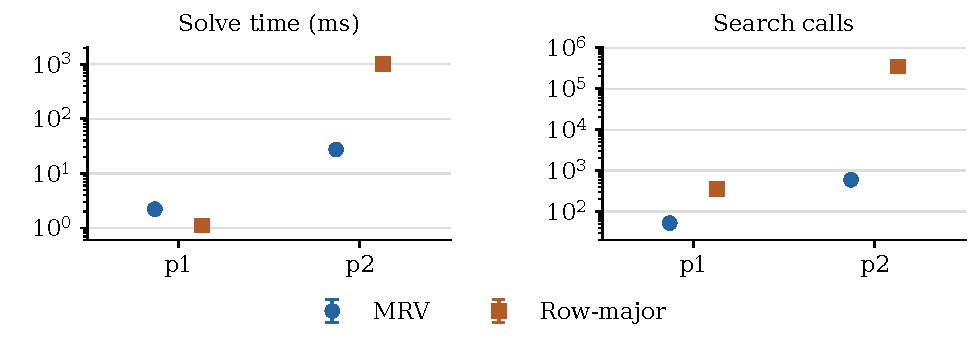
\includegraphics[width=\linewidth]{figures/sudoku-ordering.pdf}
\caption{Ordering comparison from the same saved runs. Both vertical axes are logarithmic. Points are medians; whiskers show the observed minimum and maximum, not confidence intervals. Deterministic node counts have zero range.}\label{fig:ordering}
\end{figure}
On p2, row-major visits about 588 times as many nodes and takes about 37 times as long as MRV. On p1, row-major is faster despite more nodes: MRV's candidate scans have overhead. These results illustrate a trade-off on two inputs, not general superiority. The unsatisfiable input fails immediately at the root and does not test deep unsatisfiable search.

\subsubsection{Theoretical A* analysis}
A state is a consistent partial board; an action assigns one legal digit to one blank, at cost one. The goal is a complete valid board. A* orders states using $f=g+h$ \cite{astar}. Choose $h$ as the number of blanks remaining. It is admissible and consistent: any completion requires one action per blank, and each action reduces $h$ by one. With $m$ initial blanks, $g+h=m$ at every reachable state, so this heuristic cannot rank branches. FIFO tie-breaking behaves breadth first and can retain an exponentially large frontier, whereas depth-first backtracking retains a path. A* was analysed, not implemented or benchmarked.

\clearpage
\subsection{Worked output and interpretation}\label{part1-end}
Figure~\ref{fig:gui} places an unsatisfiable input beside the actual interactive p2 result. The left grid has no repeated digits, but its upper-left blank has no legal candidate, so the solver reports failure at the root. In the right image, the 25 givens remain black and the 56 completed cells are blue. The displayed 593 placements include 537 undone attempts: $593-537=56$ retained assignments. The 594 nodes count the root plus those 593 attempted child states. These counters agree with the saved MRV run; interactive elapsed time is a separate observation.
\begin{figure}[H]\centering
\begin{minipage}[t]{.485\linewidth}\centering
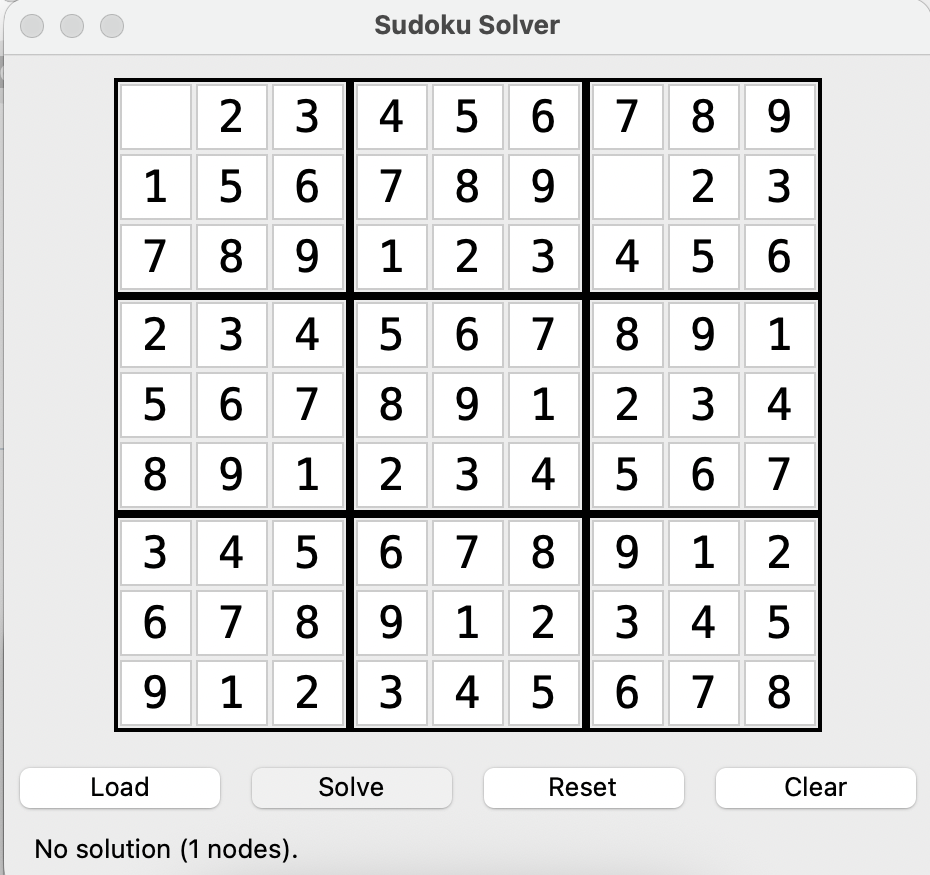
\includegraphics[width=\linewidth]{figures/sudoku-gui-no-solution.png}\\[-2pt]
{\small (a) Unsatisfiable input: 1 node}
\end{minipage}\hfill
\begin{minipage}[t]{.485\linewidth}\centering
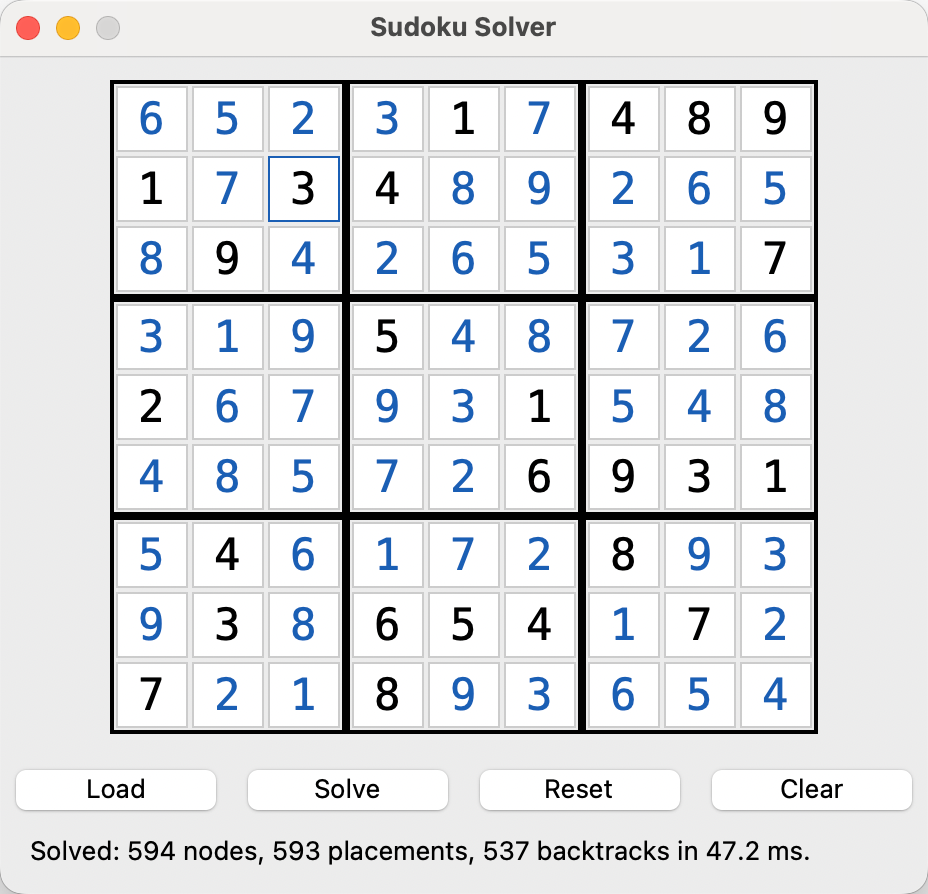
\includegraphics[width=\linewidth]{figures/sudoku-gui-p2.png}\\[-2pt]
{\small (b) p2 solved: 594 nodes}
\end{minipage}
\caption{Two actual outcomes in the Sudoku GUI. The left status reports “No solution (1 nodes)”; 47.2 ms in the right image belongs to that interactive run, while the experiment uses the five-run medians in Table~1.}\label{fig:gui}
\end{figure}
\subsubsection{Strengths, limitations and alternatives}
The method is complete, deterministic and easy to inspect; simple undo avoids domain-restoration errors. However, locally legal assignments may fail much later, and MRV selection scans can cost more than they save. Forward checking would maintain peer domains after assignments instead of recomputing them during selection; it may detect failure before another recursive call. AC-3 can remove unsupported values more widely, at added propagation cost \cite{filtering}. None of these alternatives was measured, so their performance here remains untested. Larger and externally sourced test sets, especially nontrivial unsatisfiable cases, would strengthen the evaluation; the five current inputs do not establish general performance.

\clearpage
\section{Part 2A/B: General lunar model}\label{part2-start}
\subsection{Types, state and action decisions}
The domain declares \texttt{:strips} and \texttt{:typing} \cite{spec}. Types are \texttt{rover}, \texttt{lander} and \texttt{waypoint}. Static predicates \texttt{belongs-to}, \texttt{lander-at} and \texttt{connected} encode ownership, fixed landing sites and directed roads. Dynamic predicates \texttt{aboard} and \texttt{rover-at} distinguish undeployed and deployed rovers. All action arguments are parameters; no rover, lander or waypoint identifier is hard-coded.

The eight schemas are deploy, move, capture-image, perform-scan, transmit-image, transmit-scan, collect-sample and store-sample. Deployment requires the rover aboard its own lander, removes \texttt{aboard} and creates its first waypoint location at that lander's site. Move requires an explicitly directed edge and replaces the old location. No action relocates a lander. Initial states are assumed to contain coherent ownership and locations.

\begin{table}[H]\centering
\caption{Capacity representation and the action that releases each resource.}
\begin{tabularx}{\linewidth}{@{}p{.21\linewidth}YY@{}}
\toprule
\textbf{Free token} & \textbf{Consumed by} & \textbf{Released by}\\
\midrule
\texttt{memory-free} & Capture image or scan; one shared unsent-data slot & Transmit the held image or scan to the rover's own lander\\
\texttt{sample-free} & Collect one sample; independent of data memory & Store that sample at the rover's own lander\\
\texttt{storage-free} & Store one sample in a lander & Never; no unload/discard action exists\\
\bottomrule
\end{tabularx}
\end{table}
The carrying predicates retain the source waypoint. Acquisition alone does not achieve a goal: only transmission adds \texttt{image-saved}/\texttt{scan-saved}, and only storage adds \texttt{sample-stored}. Transmission requires held data and the receiving lander's ownership, but no proximity or prior visit: it is wireless. Storage additionally requires the rover and its own lander at the same current waypoint. Thus a sample must physically return home even if its source waypoint differs from the storage location.

\subsection{Mission setup and goal destinations}
Mission 1 fixes L1 at WP1 with R1 aboard; the six supplied directed edges are retained. Mission 2 fixes L1 and deployed R1 at WP2. Its second lander L2 is placed at WP1 with R2 aboard; that unspecified landing-site choice is permitted by the task. Figure~\ref{fig:map} shows its nine directed edges.
\begin{table}[H]\centering
\caption{Scientific goals, expressed as source waypoint and receiving lander.}
\begin{tabularx}{\linewidth}{@{}llYYY@{}}
\toprule
\textbf{Mission} & \textbf{Lander} & \textbf{Image} & \textbf{Scan} & \textbf{Sample}\\
\midrule
1 & L1 & WP5 & WP3 & WP1\\
2 and 3 & L1 & WP3 & WP6 & WP5\\
2 and 3 & L2 & WP2 & WP4 & WP1\\
\bottomrule
\end{tabularx}
\end{table}
Because R1 belongs only to L1 and R2 only to L2, the destination named in a goal determines which rover can satisfy it. The same domain is used unchanged for Missions 1 and 2; problem files contain their different objects, initial states and goals.

\clearpage
\subsection{Planning results and validation}
\begin{figure}[H]\centering
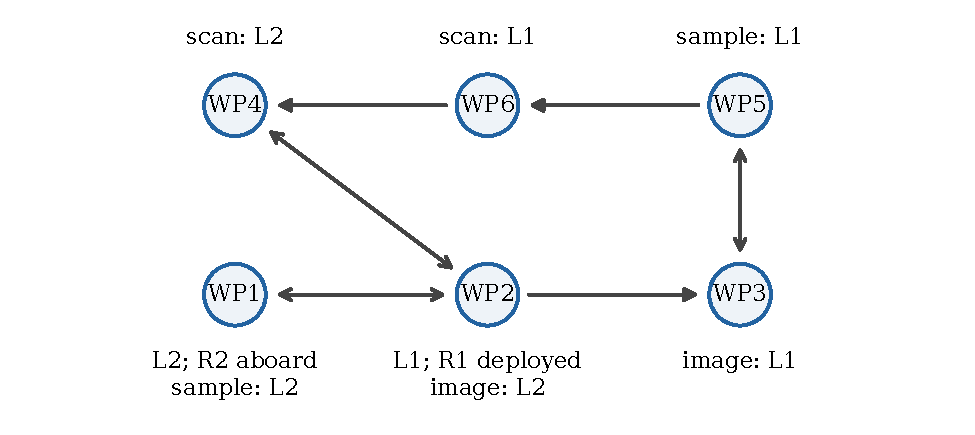
\includegraphics[width=\linewidth]{figures/mission2-map.pdf}
\caption{Mission 2 connectivity and initial placement, read directly from its PDDL. A double-headed arrow denotes both directed facts; all other arrows are one-way. Item labels name the receiving lander. Mission 3 retains this map, placement and all six goals.}\label{fig:map}
\end{figure}
Testing used Pyperplan 2.1, greedy best-first search and the hFF heuristic \cite{pyperplan}. Each saved plan was replayed against a separate implementation of the specification's preconditions and effects; merely reaching a planner goal was not treated as sufficient.
\begin{table}[H]\centering
\caption{Saved planning outcomes. A plan length is not an optimality claim.}
\begin{tabularx}{\linewidth}{@{}lrrrY@{}}
\toprule
\textbf{Mission} & \textbf{Actions} & \textbf{Goals met} & \textbf{Room moves} & \textbf{Replay}\\
\midrule
1 & 10 & 3/3 & 0 & All steps checked\\
2 & 20 & 6/6 & 0 & All steps checked\\
3 & 24 & 6/6 & 4 & All steps checked\\
\bottomrule
\end{tabularx}
\end{table}
Mission 1 includes collection and storage of the WP1 sample, scanning WP3 and later transmitting from WP5, then acquiring and sending the WP5 image. In Mission 2, R1 acquires the WP3 image and transmits from WP5, later carries a WP5 sample home to WP2, and sends the WP6 scan from WP2. These steps expose the distinction between source and current waypoint, wireless data transfer and physical sample return. Each acquisition is followed by the required transmission or storage before its goal is counted.

The base checks compare 2,496 typed action instances in 16 constructed coherent states. They include undeployed actions, one-way travel, removal of old locations, shared image/scan memory, release after transmission, independent sample capacity, foreign-lander transfers, remote storage and full lander storage. The directed edge sets are checked exactly (six for Mission 1, nine for Mission 2). These checks exercise both allowed and forbidden actions.

Generality was tested without changing the domain: the Mission 2 objects were renamed, a third rover/lander and an extra image goal were added, and a 23-action plan achieved the resulting goals. This supports parameter generality on a further instance; neither that test nor the finite state checks prove correctness on every possible instance or establish shortest plans.

\clearpage
\section{Part 2C: Astronaut extension}
\subsection{Additional state and genuine action restrictions}
New types are \texttt{astronaut} and \texttt{room}. Predicates \texttt{astronaut-belongs-to}/\texttt{room-of} record ownership, \texttt{docking-bay}/\texttt{control-room} record roles, and \texttt{astronaut-at} records location. Each lander's distinct rooms have two-way \texttt{room-connected} links.

The \texttt{move-astronaut} schema requires the source location, adjacency and ownership of both rooms by the astronaut's lander. It replaces the old location. Thus even a cross-lander adjacency fact cannot permit entry to another lander.
\begin{table}[H]\centering
\caption{Added preconditions; the original rover preconditions and effects remain.}
\begin{tabularx}{\linewidth}{@{}p{.34\linewidth}Y@{}}
\toprule
\textbf{Action group} & \textbf{Required astronaut presence}\\
\midrule
Deploy; store-sample & An astronaut belonging to the receiving lander, in that lander's docking bay\\
Transmit-image; transmit-scan & An astronaut belonging to the receiving lander, in that lander's control room\\
Move; acquire data/sample & No added astronaut-location requirement\\
\bottomrule
\end{tabularx}
\end{table}
Mission 3 preserves Mission 2's rover/lander setup, directed roads and six goals. Alice belongs to L1 and initially occupies its docking bay; Bob belongs to L2 and initially occupies its control room. The changes to applicability therefore require real room movements, rather than recording decorative astronaut facts.

\subsection{Dependency evidence from the saved 24-action plan}
\begin{table}[H]\centering
\caption{Astronaut moves and enabled actions in the saved Mission 3 plan.}
\begin{tabularx}{\linewidth}{@{}rp{.33\linewidth}Y@{}}
\toprule
\textbf{Step} & \textbf{Astronaut move} & \textbf{Later action enabled}\\
\midrule
1 & Bob: control $\to$ docking & R2 deploys at step 2; stores its WP1 sample at step 4\\
8 & Bob: docking $\to$ control & R2 transmits the WP2 image at step 9 and WP4 scan at step 11\\
17 & Alice: docking $\to$ control & R1 transmits the WP3 image at step 18 and WP6 scan at step 22\\
23 & Alice: control $\to$ docking & R1 stores the WP5 sample at L1/WP2 at step 24\\
\bottomrule
\end{tabularx}
\end{table}
Deployment at step 2 is initially inapplicable: Bob must first leave the control room. A different lander's astronaut or room cannot substitute. Plan ordering can vary; this is one saved valid sequence, not a shortest-plan claim.

\subsection{Validation and limits}
In 23 constructed coherent states, 24,380 typed action instances are checked: 180 permitted instances have correct effects and 24,200 forbidden instances are rejected. Cases include wrong astronauts/rooms, cross-lander movement, co-located landers and inherited capacities. Mission 3 replay verifies both astronauts move and all restricted actions have matching presence. Base Missions 1/2 are rechecked. This assumes coherent initial states; it is not exhaustive reachability analysis.\label{part2-end}

\clearpage
\begin{thebibliography}{9}\label{references-start}
\bibitem{spec} F29AI teaching team. \emph{Coursework 1: Search and Automated Planning}, 2026. Supplied specification, pp.~2, 4--10 and 13--17.
\bibitem{csp} S. Russell and P. Norvig. \emph{Constraint Satisfaction Problems}, Chapter 5 teaching slides, especially slides 3, 7 and 12--15. \url{https://aima.cs.berkeley.edu/4th-ed/slides-pdf/chapter05.pdf}
\bibitem{backtracking} UC Berkeley CS188. \emph{2.2 Solving Constraint Satisfaction Problems}. \url{https://inst.eecs.berkeley.edu/~cs188/textbook/csp/solving.html}
\bibitem{ordering} UC Berkeley CS188. \emph{2.4 Ordering}. \url{https://inst.eecs.berkeley.edu/~cs188/textbook/csp/ordering.html}
\bibitem{filtering} UC Berkeley CS188. \emph{2.3 Filtering}. \url{https://inst.eecs.berkeley.edu/~cs188/textbook/csp/filtering.html}
\bibitem{astar} UC Berkeley CS188. \emph{1.4 Informed Search}. \url{https://inst.eecs.berkeley.edu/~cs188/textbook/search/informed.html}
\bibitem{pyperplan} Pyperplan contributors. \emph{Pyperplan}, version 2.1. \url{https://github.com/aibasel/pyperplan}
\end{thebibliography}
\subsection*{Experiment and figure records}
The Sudoku table and comparison plot use \path{reference/part1b/results/benchmark.json} and \path{reference/part1b/results/benchmark_rowmajor.json}. The measured solver SHA-256 is \texttt{7eed993d133f22a47d3858794d5d196a2c0fce9b7663c5f01d6beb024540d281}. The interface figure is the actual interactive p2 screenshot supplied during rehearsal; its timings are kept separate from the benchmark.

The map is drawn from \path{PDDL/PartA&B/mission2.pddl}. Planning results and step references use \path{evidence/base-pddl/} and \path{evidence/part2c/}, including their plans and validation JSON. They record the data and validation conditions behind the report. Figure scripts do not overwrite those records.
\end{document}
